\documentclass[a4paper, 11pt, twocolumn]{report}

%%%%%%%%%%%%%%%%%%%%%%%%%%%%%%%%%
% PACKAGE IMPORTS
%%%%%%%%%%%%%%%%%%%%%%%%%%%%%%%%%


\usepackage[tmargin=2cm,rmargin=1in,lmargin=1in,margin=0.85in,bmargin=2cm,footskip=.2in]{geometry}
\usepackage{amsmath,amsfonts,amsthm,amssymb,mathtools}
\usepackage[varbb]{newpxmath}
\usepackage{xfrac}
\usepackage[makeroom]{cancel}
\usepackage{mathtools}
\usepackage{bookmark}
\usepackage{enumitem}
\usepackage{hyperref,theoremref}
\hypersetup{
	pdftitle={Assignment},
	colorlinks=true, linkcolor=doc!90,
	bookmarksnumbered=true,
	bookmarksopen=true
}
\usepackage[most,many,breakable]{tcolorbox}
\usepackage{xcolor}
\usepackage{varwidth}
\usepackage{varwidth}
\usepackage{etoolbox}
%\usepackage{authblk}
\usepackage{nameref}
\usepackage{multicol,array}
\usepackage{tikz-cd}
\usepackage[ruled,vlined,linesnumbered]{algorithm2e}
\usepackage{comment} % enables the use of multi-line comments (\ifx \fi) 
\usepackage{import}
\usepackage{xifthen}
\usepackage{pdfpages}
\usepackage{transparent}
\usepackage{circuitikz}
\usepackage{graphicx}
\usepackage{fancyhdr}
\usepackage[version=4]{mhchem}
\usepackage{chemstyle}
\usepackage[danish]{babel}
\usepackage{gensymb}
\usepackage{mhchem}
\usepackage{wrapfig}
\usepackage[export]{adjustbox}
\usepackage{chemfig}


\newread\tmp

\newcommand{\quickcharcount}[1]{%
  \immediate\write18{texcount -1 -sum -merge -char #1.tex > #1-chars.sum}%
  \openin\tmp=#1-chars.sum%
  \read\tmp to \thechar%
  \closein\tmp%
}

\newcommand{\quickwordcount}[1]{%
  \immediate\write18{texcount -1 -sum -merge #1.tex > #1-words.sum}%
  \openin\tmp=#1-words.sum%
  \read\tmp to \theword%
  \closein\tmp%
}


\newcommand\mycommfont[1]{\footnotesize\ttfamily\textcolor{blue}{#1}}
\SetCommentSty{mycommfont}
\newcommand{\incfig}[1]{%
    \def\svgwidth{\columnwidth}
    \import{./figures/}{#1.pdf_tex}
}

\usepackage{tikzsymbols}
\renewcommand\qedsymbol{$\Laughey$}


\mathcode`\*="8000
{\catcode`\*\active\gdef*{\cdot}}

%\usepackage{import}
%\usepackage{xifthen}
%\usepackage{pdfpages}
%\usepackage{transparent}


%%%%%%%%%%%%%%%%%%%%%%%%%%%%%%
% SELF MADE COLORS
%%%%%%%%%%%%%%%%%%%%%%%%%%%%%%



\definecolor{myg}{RGB}{56, 140, 70}
\definecolor{myb}{RGB}{45, 111, 177}
\definecolor{myr}{RGB}{199, 68, 64}
\definecolor{mytheorembg}{HTML}{F2F2F9}
\definecolor{mytheoremfr}{HTML}{00007B}
\definecolor{mylenmabg}{HTML}{FFFAF8}
\definecolor{mylenmafr}{HTML}{983b0f}
\definecolor{mypropbg}{HTML}{f2fbfc}
\definecolor{mypropfr}{HTML}{191971}
\definecolor{myexamplebg}{HTML}{F2FBF8}
\definecolor{myexamplefr}{HTML}{88D6D1}
\definecolor{myexampleti}{HTML}{2A7F7F}
\definecolor{mydefinitbg}{HTML}{E5E5FF}
\definecolor{mydefinitfr}{HTML}{3F3FA3}
\definecolor{notesgreen}{RGB}{0,162,0}
\definecolor{myp}{RGB}{197, 92, 212}
\definecolor{mygr}{HTML}{2C3338}
\definecolor{myred}{RGB}{127,0,0}
\definecolor{myyellow}{RGB}{169,121,69}
\definecolor{myexercisebg}{HTML}{F2FBF8}
\definecolor{myexercisefg}{HTML}{88D6D1}


%%%%%%%%%%%%%%%%%%%%%%%%%%%%
% TCOLORBOX SETUPS
%%%%%%%%%%%%%%%%%%%%%%%%%%%%

\setlength{\parindent}{0.5cm}
%================================
% THEOREM BOX
%================================

\tcbuselibrary{theorems,skins,hooks}
\newtcbtheorem[number within=section]{Theorem}{Theorem}
{%
	enhanced,
	breakable,
	colback = mytheorembg,
	frame hidden,
	boxrule = 0sp,
	borderline west = {2pt}{0pt}{mytheoremfr},
	sharp corners,
	detach title,
	before upper = \tcbtitle\par\smallskip,
	coltitle = mytheoremfr,
	fonttitle = \bfseries\sffamily,
	description font = \mdseries,
	separator sign none,
	segmentation style={solid, mytheoremfr},
}
{th}

\tcbuselibrary{theorems,skins,hooks}
\newtcbtheorem[number within=chapter]{theorem}{Theorem}
{%
	enhanced,
	breakable,
	colback = mytheorembg,
	frame hidden,
	boxrule = 0sp,
	borderline west = {2pt}{0pt}{mytheoremfr},
	sharp corners,
	detach title,
	before upper = \tcbtitle\par\smallskip,
	coltitle = mytheoremfr,
	fonttitle = \bfseries\sffamily,
	description font = \mdseries,
	separator sign none,
	segmentation style={solid, mytheoremfr},
}
{th}


\tcbuselibrary{theorems,skins,hooks}
\newtcolorbox{Theoremcon}
{%
	enhanced
	,breakable
	,colback = mytheorembg
	,frame hidden
	,boxrule = 0sp
	,borderline west = {2pt}{0pt}{mytheoremfr}
	,sharp corners
	,description font = \mdseries
	,separator sign none
}

%================================
% Corollery
%================================
\tcbuselibrary{theorems,skins,hooks}
\newtcbtheorem[number within=section]{Corollary}{Corollary}
{%
	enhanced
	,breakable
	,colback = myp!10
	,frame hidden
	,boxrule = 0sp
	,borderline west = {2pt}{0pt}{myp!85!black}
	,sharp corners
	,detach title
	,before upper = \tcbtitle\par\smallskip
	,coltitle = myp!85!black
	,fonttitle = \bfseries\sffamily
	,description font = \mdseries
	,separator sign none
	,segmentation style={solid, myp!85!black}
}
{th}
\tcbuselibrary{theorems,skins,hooks}
\newtcbtheorem[number within=chapter]{corollary}{Corollary}
{%
	enhanced
	,breakable
	,colback = myp!10
	,frame hidden
	,boxrule = 0sp
	,borderline west = {2pt}{0pt}{myp!85!black}
	,sharp corners
	,detach title
	,before upper = \tcbtitle\par\smallskip
	,coltitle = myp!85!black
	,fonttitle = \bfseries\sffamily
	,description font = \mdseries
	,separator sign none
	,segmentation style={solid, myp!85!black}
}
{th}


%================================
% LENMA
%================================

\tcbuselibrary{theorems,skins,hooks}
\newtcbtheorem[number within=section]{Lenma}{Lenma}
{%
	enhanced,
	breakable,
	colback = mylenmabg,
	frame hidden,
	boxrule = 0sp,
	borderline west = {2pt}{0pt}{mylenmafr},
	sharp corners,
	detach title,
	before upper = \tcbtitle\par\smallskip,
	coltitle = mylenmafr,
	fonttitle = \bfseries\sffamily,
	description font = \mdseries,
	separator sign none,
	segmentation style={solid, mylenmafr},
}
{th}

\tcbuselibrary{theorems,skins,hooks}
\newtcbtheorem[number within=chapter]{lenma}{Lenma}
{%
	enhanced,
	breakable,
	colback = mylenmabg,
	frame hidden,
	boxrule = 0sp,
	borderline west = {2pt}{0pt}{mylenmafr},
	sharp corners,
	detach title,
	before upper = \tcbtitle\par\smallskip,
	coltitle = mylenmafr,
	fonttitle = \bfseries\sffamily,
	description font = \mdseries,
	separator sign none,
	segmentation style={solid, mylenmafr},
}
{th}


%================================
% PROPOSITION
%================================

\tcbuselibrary{theorems,skins,hooks}
\newtcbtheorem[number within=section]{Prop}{Proposition}
{%
	enhanced,
	breakable,
	colback = mypropbg,
	frame hidden,
	boxrule = 0sp,
	borderline west = {2pt}{0pt}{mypropfr},
	sharp corners,
	detach title,
	before upper = \tcbtitle\par\smallskip,
	coltitle = mypropfr,
	fonttitle = \bfseries\sffamily,
	description font = \mdseries,
	separator sign none,
	segmentation style={solid, mypropfr},
}
{th}

\tcbuselibrary{theorems,skins,hooks}
\newtcbtheorem[number within=chapter]{prop}{Proposition}
{%
	enhanced,
	breakable,
	colback = mypropbg,
	frame hidden,
	boxrule = 0sp,
	borderline west = {2pt}{0pt}{mypropfr},
	sharp corners,
	detach title,
	before upper = \tcbtitle\par\smallskip,
	coltitle = mypropfr,
	fonttitle = \bfseries\sffamily,
	description font = \mdseries,
	separator sign none,
	segmentation style={solid, mypropfr},
}
{th}


%================================
% CLAIM
%================================

\tcbuselibrary{theorems,skins,hooks}
\newtcbtheorem[number within=section]{claim}{Claim}
{%
	enhanced
	,breakable
	,colback = myg!10
	,frame hidden
	,boxrule = 0sp
	,borderline west = {2pt}{0pt}{myg}
	,sharp corners
	,detach title
	,before upper = \tcbtitle\par\smallskip
	,coltitle = myg!85!black
	,fonttitle = \bfseries\sffamily
	,description font = \mdseries
	,separator sign none
	,segmentation style={solid, myg!85!black}
}
{th}



%================================
% Exercise
%================================

\tcbuselibrary{theorems,skins,hooks}
\newtcbtheorem[number within=section]{Exercise}{Exercise}
{%
	enhanced,
	breakable,
	colback = myexercisebg,
	frame hidden,
	boxrule = 0sp,
	borderline west = {2pt}{0pt}{myexercisefg},
	sharp corners,
	detach title,
	before upper = \tcbtitle\par\smallskip,
	coltitle = myexercisefg,
	fonttitle = \bfseries\sffamily,
	description font = \mdseries,
	separator sign none,
	segmentation style={solid, myexercisefg},
}
{th}

\tcbuselibrary{theorems,skins,hooks}
\newtcbtheorem[number within=chapter]{exercise}{Exercise}
{%
	enhanced,
	breakable,
	colback = myexercisebg,
	frame hidden,
	boxrule = 0sp,
	borderline west = {2pt}{0pt}{myexercisefg},
	sharp corners,
	detach title,
	before upper = \tcbtitle\par\smallskip,
	coltitle = myexercisefg,
	fonttitle = \bfseries\sffamily,
	description font = \mdseries,
	separator sign none,
	segmentation style={solid, myexercisefg},
}
{th}

%================================
% EXAMPLE BOX
%================================

\newtcbtheorem[number within=section]{Example}{Eksempel}
{%
	colback = myexamplebg
	,breakable
	,colframe = myexamplefr
	,coltitle = myexampleti
	,boxrule = 1pt
	,sharp corners
	,detach title
	,before upper=\tcbtitle\par\smallskip
	,fonttitle = \bfseries
	,description font = \mdseries
	,separator sign none
	,description delimiters parenthesis
}
{ex}

\newtcbtheorem[number within=chapter]{example}{Example}
{%
	colback = myexamplebg
	,breakable
	,colframe = myexamplefr
	,coltitle = myexampleti
	,boxrule = 1pt
	,sharp corners
	,detach title
	,before upper=\tcbtitle\par\smallskip
	,fonttitle = \bfseries
	,description font = \mdseries
	,separator sign none
	,description delimiters parenthesis
}
{ex}

%================================
% DEFINITION BOX
%================================

\newtcbtheorem[number within=section]{Definition}{Definition}{enhanced,
	before skip=2mm,after skip=2mm, colback=red!5,colframe=red!80!black,boxrule=0.5mm,
	attach boxed title to top left={xshift=1cm,yshift*=1mm-\tcboxedtitleheight}, varwidth boxed title*=-3cm,
	boxed title style={frame code={
					\path[fill=tcbcolback]
					([yshift=-1mm,xshift=-1mm]frame.north west)
					arc[start angle=0,end angle=180,radius=1mm]
					([yshift=-1mm,xshift=1mm]frame.north east)
					arc[start angle=180,end angle=0,radius=1mm];
					\path[left color=tcbcolback!60!black,right color=tcbcolback!60!black,
						middle color=tcbcolback!80!black]
					([xshift=-2mm]frame.north west) -- ([xshift=2mm]frame.north east)
					[rounded corners=1mm]-- ([xshift=1mm,yshift=-1mm]frame.north east)
					-- (frame.south east) -- (frame.south west)
					-- ([xshift=-1mm,yshift=-1mm]frame.north west)
					[sharp corners]-- cycle;
				},interior engine=empty,
		},
	fonttitle=\bfseries,
	title={#2},#1}{def}
\newtcbtheorem[number within=chapter]{definition}{Definition}{enhanced,
	before skip=2mm,after skip=2mm, colback=red!5,colframe=red!80!black,boxrule=0.5mm,
	attach boxed title to top left={xshift=1cm,yshift*=1mm-\tcboxedtitleheight}, varwidth boxed title*=-3cm,
	boxed title style={frame code={
					\path[fill=tcbcolback]
					([yshift=-1mm,xshift=-1mm]frame.north west)
					arc[start angle=0,end angle=180,radius=1mm]
					([yshift=-1mm,xshift=1mm]frame.north east)
					arc[start angle=180,end angle=0,radius=1mm];
					\path[left color=tcbcolback!60!black,right color=tcbcolback!60!black,
						middle color=tcbcolback!80!black]
					([xshift=-2mm]frame.north west) -- ([xshift=2mm]frame.north east)
					[rounded corners=1mm]-- ([xshift=1mm,yshift=-1mm]frame.north east)
					-- (frame.south east) -- (frame.south west)
					-- ([xshift=-1mm,yshift=-1mm]frame.north west)
					[sharp corners]-- cycle;
				},interior engine=empty,
		},
	fonttitle=\bfseries,
	title={#2},#1}{def}



%================================
% Question BOX
%================================

\makeatletter
\newtcbtheorem{question}{Spørgsmål}{enhanced,
	breakable,
	colback=white,
	colframe=myb!80!black,
	attach boxed title to top left={yshift*=-\tcboxedtitleheight},
	fonttitle=\bfseries,
	title={#2},
	boxed title size=title,
	boxed title style={%
			sharp corners,
			rounded corners=northwest,
			colback=tcbcolframe,
			boxrule=0pt,
		},
	underlay boxed title={%
			\path[fill=tcbcolframe] (title.south west)--(title.south east)
			to[out=0, in=180] ([xshift=5mm]title.east)--
			(title.center-|frame.east)
			[rounded corners=\kvtcb@arc] |-
			(frame.north) -| cycle;
		},
	#1
}{def}
\makeatother

%================================
% SOLUTION BOX
%================================

\makeatletter
\newtcolorbox{solution}{enhanced,
	breakable,
	colback=white,
	colframe=myg!80!black,
	attach boxed title to top left={yshift*=-\tcboxedtitleheight},
	title=Solution,
	boxed title size=title,
	boxed title style={%
			sharp corners,
			rounded corners=northwest,
			colback=tcbcolframe,
			boxrule=0pt,
		},
	underlay boxed title={%
			\path[fill=tcbcolframe] (title.south west)--(title.south east)
			to[out=0, in=180] ([xshift=5mm]title.east)--
			(title.center-|frame.east)
			[rounded corners=\kvtcb@arc] |-
			(frame.north) -| cycle;
		},
}
\makeatother


%================================
% NOTE BOX
%================================

\usetikzlibrary{arrows,calc,shadows.blur}
\tcbuselibrary{skins}
\newtcolorbox{note}[1][]{%
	enhanced jigsaw,
	colback=gray!20!white,%
	colframe=gray!80!black,
	size=small,
	boxrule=1pt,
	title=\textbf{Note:-},
	halign title=flush center,
	coltitle=black,
	breakable,
	drop shadow=black!50!white,
	attach boxed title to top left={xshift=1cm,yshift=-\tcboxedtitleheight/2,yshifttext=-\tcboxedtitleheight/2},
	minipage boxed title=1.5cm,
	boxed title style={%
			colback=white,
			size=fbox,
			boxrule=1pt,
			boxsep=2pt,
			underlay={%
					\coordinate (dotA) at ($(interior.west) + (-0.5pt,0)$);
					\coordinate (dotB) at ($(interior.east) + (0.5pt,0)$);
					\begin{scope}
						\clip (interior.north west) rectangle ([xshift=3ex]interior.east);
						\filldraw [white, blur shadow={shadow opacity=60, shadow yshift=-.75ex}, rounded corners=2pt] (interior.north west) rectangle (interior.south east);
					\end{scope}
					\begin{scope}[gray!80!black]
						\fill (dotA) circle (2pt);
						\fill (dotB) circle (2pt);
					\end{scope}
				},
		},
	#1,
}

%%%%%%%%%%%%%%%%%%%%%%%%%%%%%%
% SELF MADE COMMANDS
%%%%%%%%%%%%%%%%%%%%%%%%%%%%%%


\newcommand{\thm}[2]{\begin{Theorem}{#1}{}#2\end{Theorem}}
\newcommand{\cor}[2]{\begin{Corollary}{#1}{}#2\end{Corollary}}
\newcommand{\mlenma}[2]{\begin{Lenma}{#1}{}#2\end{Lenma}}
\newcommand{\mprop}[2]{\begin{Prop}{#1}{}#2\end{Prop}}
\newcommand{\clm}[3]{\begin{claim}{#1}{#2}#3\end{claim}}
\newcommand{\wc}[2]{\begin{wconc}{#1}{}\setlength{\parindent}{1cm}#2\end{wconc}}
\newcommand{\thmcon}[1]{\begin{Theoremcon}{#1}\end{Theoremcon}}
\newcommand{\ex}[2]{\begin{Example}{#1}{}#2\end{Example}}
\newcommand{\dfn}[2]{\begin{Definition}[colbacktitle=red!75!black]{#1}{}#2\end{Definition}}
\newcommand{\dfnc}[2]{\begin{definition}[colbacktitle=red!75!black]{#1}{}#2\end{definition}}
\newcommand{\qs}[2]{\begin{question}{#1}{}#2\end{question}}
\newcommand{\pf}[2]{\begin{myproof}[#1]#2\end{myproof}}
\newcommand{\nt}[1]{\begin{note}#1\end{note}}

\newcommand*\circled[1]{\tikz[baseline=(char.base)]{
		\node[shape=circle,draw,inner sep=1pt] (char) {#1};}}
\newcommand\getcurrentref[1]{%
	\ifnumequal{\value{#1}}{0}
	{??}
	{\the\value{#1}}%
}
\newcommand{\getCurrentSectionNumber}{\getcurrentref{section}}
\newenvironment{myproof}[1][\proofname]{%
	\proof[\bfseries #1: ]%
}{\endproof}

\newcommand{\mclm}[2]{\begin{myclaim}[#1]#2\end{myclaim}}
\newenvironment{myclaim}[1][\claimname]{\proof[\bfseries #1: ]}{}

\newcounter{mylabelcounter}

\makeatletter
\newcommand{\setword}[2]{%
	\phantomsection
	#1\def\@currentlabel{\unexpanded{#1}}\label{#2}%
}
\makeatother




\tikzset{
	symbol/.style={
			draw=none,
			every to/.append style={
					edge node={node [sloped, allow upside down, auto=false]{$#1$}}}
		}
}


% deliminators
\DeclarePairedDelimiter{\abs}{\lvert}{\rvert}
\DeclarePairedDelimiter{\norm}{\lVert}{\rVert}

\DeclarePairedDelimiter{\ceil}{\lceil}{\rceil}
\DeclarePairedDelimiter{\floor}{\lfloor}{\rfloor}
\DeclarePairedDelimiter{\round}{\lfloor}{\rceil}

\newsavebox\diffdbox
\newcommand{\slantedromand}{{\mathpalette\makesl{d}}}
\newcommand{\makesl}[2]{%
\begingroup
\sbox{\diffdbox}{$\mathsurround=0pt#1\mathrm{#2}$}%
\pdfsave
\pdfsetmatrix{1 0 0.2 1}%
\rlap{\usebox{\diffdbox}}%
\pdfrestore
\hskip\wd\diffdbox
\endgroup
}
\newcommand{\dd}[1][]{\ensuremath{\mathop{}\!\ifstrempty{#1}{%
\slantedromand\@ifnextchar^{\hspace{0.2ex}}{\hspace{0.1ex}}}%
{\slantedromand\hspace{0.2ex}^{#1}}}}
\ProvideDocumentCommand\dv{o m g}{%
  \ensuremath{%
    \IfValueTF{#3}{%
      \IfNoValueTF{#1}{%
        \frac{\dd #2}{\dd #3}%
      }{%
        \frac{\dd^{#1} #2}{\dd #3^{#1}}%
      }%
    }{%
      \IfNoValueTF{#1}{%
        \frac{\dd}{\dd #2}%
      }{%
        \frac{\dd^{#1}}{\dd #2^{#1}}%
      }%
    }%
  }%
}
\providecommand*{\pdv}[3][]{\frac{\partial^{#1}#2}{\partial#3^{#1}}}
%  - others
\DeclareMathOperator{\Lap}{\mathcal{L}}
\DeclareMathOperator{\Var}{Var} % varience
\DeclareMathOperator{\Cov}{Cov} % covarience
\DeclareMathOperator{\E}{E} % expected

% Since the amsthm package isn't loaded

% I prefer the slanted \leq
\let\oldleq\leq % save them in case they're every wanted
\let\oldgeq\geq
\renewcommand{\leq}{\leqslant}
\renewcommand{\geq}{\geqslant}

% % redefine matrix env to allow for alignment, use r as default
% \renewcommand*\env@matrix[1][r]{\hskip -\arraycolsep
%     \let\@ifnextchar\new@ifnextchar
%     \array{*\c@MaxMatrixCols #1}}


%\usepackage{framed}
%\usepackage{titletoc}
%\usepackage{etoolbox}
%\usepackage{lmodern}


%\patchcmd{\tableofcontents}{\contentsname}{\sffamily\contentsname}{}{}

%\renewenvironment{leftbar}
%{\def\FrameCommand{\hspace{6em}%
%		{\color{myyellow}\vrule width 2pt depth 6pt}\hspace{1em}}%
%	\MakeFramed{\parshape 1 0cm \dimexpr\textwidth-6em\relax\FrameRestore}\vskip2pt%
%}
%{\endMakeFramed}

%\titlecontents{chapter}
%[0em]{\vspace*{2\baselineskip}}
%{\parbox{4.5em}{%
%		\hfill\Huge\sffamily\bfseries\color{myred}\thecontentspage}%
%	\vspace*{-2.3\baselineskip}\leftbar\textsc{\small\chaptername~\thecontentslabel}\\\sffamily}
%{}{\endleftbar}
%\titlecontents{section}
%[8.4em]
%{\sffamily\contentslabel{3em}}{}{}
%{\hspace{0.5em}\nobreak\itshape\color{myred}\contentspage}
%\titlecontents{subsection}
%[8.4em]
%{\sffamily\contentslabel{3em}}{}{}  
%{\hspace{0.5em}\nobreak\itshape\color{myred}\contentspage}



%%%%%%%%%%%%%%%%%%%%%%%%%%%%%%%%%%%%%%%%%%%
% TABLE OF CONTENTS
%%%%%%%%%%%%%%%%%%%%%%%%%%%%%%%%%%%%%%%%%%%

\usepackage{tikz}
\definecolor{doc}{RGB}{0,60,110}
\usepackage{titletoc}
\contentsmargin{0cm}
\titlecontents{chapter}[3.7pc]
{\addvspace{30pt}%
	\begin{tikzpicture}[remember picture, overlay]%
		\draw[fill=doc!60,draw=doc!60] (-7,-.1) rectangle (-0.9,.5);%
		\pgftext[left,x=-3.5cm,y=0.2cm]{\color{white}\Large\sc\bfseries Kapitel\ \thecontentslabel};%
	\end{tikzpicture}\color{doc!60}\large\sc\bfseries}%
{}
{}
{\;\titlerule\;\large\sc\bfseries Side \thecontentspage
	\begin{tikzpicture}[remember picture, overlay]
		\draw[fill=doc!60,draw=doc!60] (2pt,0) rectangle (4,0.1pt);
	\end{tikzpicture}}%
\titlecontents{section}[3.7pc]
{\addvspace{2pt}}
{\contentslabel[\thecontentslabel]{2pc}}
{}
{\hfill\small \thecontentspage}
[]
\titlecontents*{subsection}[3.7pc]
{\addvspace{-1pt}\small}
{}
{}
{\ --- \small\thecontentspage}
[ \textbullet\ ][]

\makeatletter
\renewcommand{\tableofcontents}{%
	\chapter*{%
	  \vspace*{-20\p@}%
	  \begin{tikzpicture}[remember picture, overlay]%
		  \pgftext[right,x=15cm,y=0.2cm]{\color{doc!60}\Huge\sc\bfseries \contentsname};%
		  \draw[fill=doc!60,draw=doc!60] (13,-.75) rectangle (20,1);%
		  \clip (13,-.75) rectangle (20,1);
		  \pgftext[right,x=15cm,y=0.2cm]{\color{white}\Huge\sc\bfseries \contentsname};%
	  \end{tikzpicture}}%
	\@starttoc{toc}}
\makeatother

%From M275 "Topology" at SJSU
\newcommand{\id}{\mathrm{id}}
\newcommand{\taking}[1]{\xrightarrow{#1}}
\newcommand{\inv}{^{-1}}

%From M170 "Introduction to Graph Theory" at SJSU
\DeclareMathOperator{\diam}{diam}
\DeclareMathOperator{\ord}{ord}
\newcommand{\defeq}{\overset{\mathrm{def}}{=}}

%From the USAMO .tex files
\newcommand{\ts}{\textsuperscript}
\newcommand{\dg}{^\circ}
\newcommand{\ii}{\item}

% % From Math 55 and Math 145 at Harvard
% \newenvironment{subproof}[1][Proof]{%
% \begin{proof}[#1] \renewcommand{\qedsymbol}{$\blacksquare$}}%
% {\end{proof}}

\newcommand{\liff}{\leftrightarrow}
\newcommand{\lthen}{\rightarrow}
\newcommand{\opname}{\operatorname}
\newcommand{\surjto}{\twoheadrightarrow}
\newcommand{\injto}{\hookrightarrow}
\newcommand{\On}{\mathrm{On}} % ordinals
\DeclareMathOperator{\img}{im} % Image
\DeclareMathOperator{\Img}{Im} % Image
\DeclareMathOperator{\coker}{coker} % Cokernel
\DeclareMathOperator{\Coker}{Coker} % Cokernel
\DeclareMathOperator{\Ker}{Ker} % Kernel
\DeclareMathOperator{\rank}{rank}
\DeclareMathOperator{\Spec}{Spec} % spectrum
\DeclareMathOperator{\Tr}{Tr} % trace
\DeclareMathOperator{\pr}{pr} % projection
\DeclareMathOperator{\ext}{ext} % extension
\DeclareMathOperator{\pred}{pred} % predecessor
\DeclareMathOperator{\dom}{dom} % domain
\DeclareMathOperator{\ran}{ran} % range
\DeclareMathOperator{\Hom}{Hom} % homomorphism
\DeclareMathOperator{\Mor}{Mor} % morphisms
\DeclareMathOperator{\End}{End} % endomorphism

\newcommand{\eps}{\epsilon}
\newcommand{\veps}{\varepsilon}
\newcommand{\ol}{\overline}
\newcommand{\ul}{\underline}
\newcommand{\wt}{\widetilde}
\newcommand{\wh}{\widehat}
\newcommand{\vocab}[1]{\textbf{\color{blue} #1}}
\providecommand{\half}{\frac{1}{2}}
\newcommand{\dang}{\measuredangle} %% Directed angle
\newcommand{\ray}[1]{\overrightarrow{#1}}
\newcommand{\seg}[1]{\overline{#1}}
\newcommand{\arc}[1]{\wideparen{#1}}
\DeclareMathOperator{\cis}{cis}
\DeclareMathOperator*{\lcm}{lcm}
\DeclareMathOperator*{\argmin}{arg min}
\DeclareMathOperator*{\argmax}{arg max}
\newcommand{\cycsum}{\sum_{\mathrm{cyc}}}
\newcommand{\symsum}{\sum_{\mathrm{sym}}}
\newcommand{\cycprod}{\prod_{\mathrm{cyc}}}
\newcommand{\symprod}{\prod_{\mathrm{sym}}}
\newcommand{\Qed}{\begin{flushright}\qed\end{flushright}}
\newcommand{\parinn}{\setlength{\parindent}{1cm}}
\newcommand{\parinf}{\setlength{\parindent}{0cm}}
% \newcommand{\norm}{\|\cdot\|}
\newcommand{\inorm}{\norm_{\infty}}
\newcommand{\opensets}{\{V_{\alpha}\}_{\alpha\in I}}
\newcommand{\oset}{V_{\alpha}}
\newcommand{\opset}[1]{V_{\alpha_{#1}}}
\newcommand{\lub}{\text{lub}}
\newcommand{\del}[2]{\frac{\partial #1}{\partial #2}}
\newcommand{\Del}[3]{\frac{\partial^{#1} #2}{\partial^{#1} #3}}
\newcommand{\deld}[2]{\dfrac{\partial #1}{\partial #2}}
\newcommand{\Deld}[3]{\dfrac{\partial^{#1} #2}{\partial^{#1} #3}}
\newcommand{\lm}{\lambda}
\newcommand{\uin}{\mathbin{\rotatebox[origin=c]{90}{$\in$}}}
\newcommand{\usubset}{\mathbin{\rotatebox[origin=c]{90}{$\subset$}}}
\newcommand{\lt}{\left}
\newcommand{\rt}{\right}
\newcommand{\bs}[1]{\boldsymbol{#1}}
\newcommand{\exs}{\exists}
\newcommand{\st}{\strut}
\newcommand{\dps}[1]{\displaystyle{#1}}

\newcommand{\sol}{\setlength{\parindent}{0cm}\textbf{\textit{Solution:}}\setlength{\parindent}{1cm} }
\newcommand{\solve}[1]{\setlength{\parindent}{0cm}\textbf{\textit{Solution: }}\setlength{\parindent}{1cm}#1 \Qed}
% Things Lie
\newcommand{\kb}{\mathfrak b}
\newcommand{\kg}{\mathfrak g}
\newcommand{\kh}{\mathfrak h}
\newcommand{\kn}{\mathfrak n}
\newcommand{\ku}{\mathfrak u}
\newcommand{\kz}{\mathfrak z}
\DeclareMathOperator{\Ext}{Ext} % Ext functor
\DeclareMathOperator{\Tor}{Tor} % Tor functor
\newcommand{\gl}{\opname{\mathfrak{gl}}} % frak gl group
\renewcommand{\sl}{\opname{\mathfrak{sl}}} % frak sl group chktex 6

% More script letters etc.
\newcommand{\SA}{\mathcal A}
\newcommand{\SB}{\mathcal B}
\newcommand{\SC}{\mathcal C}
\newcommand{\SF}{\mathcal F}
\newcommand{\SG}{\mathcal G}
\newcommand{\SH}{\mathcal H}
\newcommand{\OO}{\mathcal O}

\newcommand{\SCA}{\mathscr A}
\newcommand{\SCB}{\mathscr B}
\newcommand{\SCC}{\mathscr C}
\newcommand{\SCD}{\mathscr D}
\newcommand{\SCE}{\mathscr E}
\newcommand{\SCF}{\mathscr F}
\newcommand{\SCG}{\mathscr G}
\newcommand{\SCH}{\mathscr H}

% Mathfrak primes
\newcommand{\km}{\mathfrak m}
\newcommand{\kp}{\mathfrak p}
\newcommand{\kq}{\mathfrak q}

% number sets
\newcommand{\RR}[1][]{\ensuremath{\ifstrempty{#1}{\mathbb{R}}{\mathbb{R}^{#1}}}}
\newcommand{\NN}[1][]{\ensuremath{\ifstrempty{#1}{\mathbb{N}}{\mathbb{N}^{#1}}}}
\newcommand{\ZZ}[1][]{\ensuremath{\ifstrempty{#1}{\mathbb{Z}}{\mathbb{Z}^{#1}}}}
\newcommand{\QQ}[1][]{\ensuremath{\ifstrempty{#1}{\mathbb{Q}}{\mathbb{Q}^{#1}}}}
\newcommand{\CC}[1][]{\ensuremath{\ifstrempty{#1}{\mathbb{C}}{\mathbb{C}^{#1}}}}
\newcommand{\PP}[1][]{\ensuremath{\ifstrempty{#1}{\mathbb{P}}{\mathbb{P}^{#1}}}}
\newcommand{\HH}[1][]{\ensuremath{\ifstrempty{#1}{\mathbb{H}}{\mathbb{H}^{#1}}}}
\newcommand{\FF}[1][]{\ensuremath{\ifstrempty{#1}{\mathbb{F}}{\mathbb{F}^{#1}}}}
% expected value
\newcommand{\EE}{\ensuremath{\mathbb{E}}}
\newcommand{\charin}{\text{ char }}
\DeclareMathOperator{\sign}{sign}
\DeclareMathOperator{\Aut}{Aut}
\DeclareMathOperator{\Inn}{Inn}
\DeclareMathOperator{\Syl}{Syl}
\DeclareMathOperator{\Gal}{Gal}
\DeclareMathOperator{\GL}{GL} % General linear group
\DeclareMathOperator{\SL}{SL} % Special linear group

%---------------------------------------
% BlackBoard Math Fonts :-
%---------------------------------------

%Captital Letters
\newcommand{\bbA}{\mathbb{A}}	\newcommand{\bbB}{\mathbb{B}}
\newcommand{\bbC}{\mathbb{C}}	\newcommand{\bbD}{\mathbb{D}}
\newcommand{\bbE}{\mathbb{E}}	\newcommand{\bbF}{\mathbb{F}}
\newcommand{\bbG}{\mathbb{G}}	\newcommand{\bbH}{\mathbb{H}}
\newcommand{\bbI}{\mathbb{I}}	\newcommand{\bbJ}{\mathbb{J}}
\newcommand{\bbK}{\mathbb{K}}	\newcommand{\bbL}{\mathbb{L}}
\newcommand{\bbM}{\mathbb{M}}	\newcommand{\bbN}{\mathbb{N}}
\newcommand{\bbO}{\mathbb{O}}	\newcommand{\bbP}{\mathbb{P}}
\newcommand{\bbQ}{\mathbb{Q}}	\newcommand{\bbR}{\mathbb{R}}
\newcommand{\bbS}{\mathbb{S}}	\newcommand{\bbT}{\mathbb{T}}
\newcommand{\bbU}{\mathbb{U}}	\newcommand{\bbV}{\mathbb{V}}
\newcommand{\bbW}{\mathbb{W}}	\newcommand{\bbX}{\mathbb{X}}
\newcommand{\bbY}{\mathbb{Y}}	\newcommand{\bbZ}{\mathbb{Z}}

%---------------------------------------
% MathCal Fonts :-
%---------------------------------------

%Captital Letters
\newcommand{\mcA}{\mathcal{A}}	\newcommand{\mcB}{\mathcal{B}}
\newcommand{\mcC}{\mathcal{C}}	\newcommand{\mcD}{\mathcal{D}}
\newcommand{\mcE}{\mathcal{E}}	\newcommand{\mcF}{\mathcal{F}}
\newcommand{\mcG}{\mathcal{G}}	\newcommand{\mcH}{\mathcal{H}}
\newcommand{\mcI}{\mathcal{I}}	\newcommand{\mcJ}{\mathcal{J}}
\newcommand{\mcK}{\mathcal{K}}	\newcommand{\mcL}{\mathcal{L}}
\newcommand{\mcM}{\mathcal{M}}	\newcommand{\mcN}{\mathcal{N}}
\newcommand{\mcO}{\mathcal{O}}	\newcommand{\mcP}{\mathcal{P}}
\newcommand{\mcQ}{\mathcal{Q}}	\newcommand{\mcR}{\mathcal{R}}
\newcommand{\mcS}{\mathcal{S}}	\newcommand{\mcT}{\mathcal{T}}
\newcommand{\mcU}{\mathcal{U}}	\newcommand{\mcV}{\mathcal{V}}
\newcommand{\mcW}{\mathcal{W}}	\newcommand{\mcX}{\mathcal{X}}
\newcommand{\mcY}{\mathcal{Y}}	\newcommand{\mcZ}{\mathcal{Z}}


%---------------------------------------
% Bold Math Fonts :-
%---------------------------------------

%Captital Letters
\newcommand{\bmA}{\boldsymbol{A}}	\newcommand{\bmB}{\boldsymbol{B}}
\newcommand{\bmC}{\boldsymbol{C}}	\newcommand{\bmD}{\boldsymbol{D}}
\newcommand{\bmE}{\boldsymbol{E}}	\newcommand{\bmF}{\boldsymbol{F}}
\newcommand{\bmG}{\boldsymbol{G}}	\newcommand{\bmH}{\boldsymbol{H}}
\newcommand{\bmI}{\boldsymbol{I}}	\newcommand{\bmJ}{\boldsymbol{J}}
\newcommand{\bmK}{\boldsymbol{K}}	\newcommand{\bmL}{\boldsymbol{L}}
\newcommand{\bmM}{\boldsymbol{M}}	\newcommand{\bmN}{\boldsymbol{N}}
\newcommand{\bmO}{\boldsymbol{O}}	\newcommand{\bmP}{\boldsymbol{P}}
\newcommand{\bmQ}{\boldsymbol{Q}}	\newcommand{\bmR}{\boldsymbol{R}}
\newcommand{\bmS}{\boldsymbol{S}}	\newcommand{\bmT}{\boldsymbol{T}}
\newcommand{\bmU}{\boldsymbol{U}}	\newcommand{\bmV}{\boldsymbol{V}}
\newcommand{\bmW}{\boldsymbol{W}}	\newcommand{\bmX}{\boldsymbol{X}}
\newcommand{\bmY}{\boldsymbol{Y}}	\newcommand{\bmZ}{\boldsymbol{Z}}
%Small Letters
\newcommand{\bma}{\boldsymbol{a}}	\newcommand{\bmb}{\boldsymbol{b}}
\newcommand{\bmc}{\boldsymbol{c}}	\newcommand{\bmd}{\boldsymbol{d}}
\newcommand{\bme}{\boldsymbol{e}}	\newcommand{\bmf}{\boldsymbol{f}}
\newcommand{\bmg}{\boldsymbol{g}}	\newcommand{\bmh}{\boldsymbol{h}}
\newcommand{\bmi}{\boldsymbol{i}}	\newcommand{\bmj}{\boldsymbol{j}}
\newcommand{\bmk}{\boldsymbol{k}}	\newcommand{\bml}{\boldsymbol{l}}
\newcommand{\bmm}{\boldsymbol{m}}	\newcommand{\bmn}{\boldsymbol{n}}
\newcommand{\bmo}{\boldsymbol{o}}	\newcommand{\bmp}{\boldsymbol{p}}
\newcommand{\bmq}{\boldsymbol{q}}	\newcommand{\bmr}{\boldsymbol{r}}
\newcommand{\bms}{\boldsymbol{s}}	\newcommand{\bmt}{\boldsymbol{t}}
\newcommand{\bmu}{\boldsymbol{u}}	\newcommand{\bmv}{\boldsymbol{v}}
\newcommand{\bmw}{\boldsymbol{w}}	\newcommand{\bmx}{\boldsymbol{x}}
\newcommand{\bmy}{\boldsymbol{y}}	\newcommand{\bmz}{\boldsymbol{z}}

%---------------------------------------
% Scr Math Fonts :-
%---------------------------------------

\newcommand{\sA}{{\mathscr{A}}}   \newcommand{\sB}{{\mathscr{B}}}
\newcommand{\sC}{{\mathscr{C}}}   \newcommand{\sD}{{\mathscr{D}}}
\newcommand{\sE}{{\mathscr{E}}}   \newcommand{\sF}{{\mathscr{F}}}
\newcommand{\sG}{{\mathscr{G}}}   \newcommand{\sH}{{\mathscr{H}}}
\newcommand{\sI}{{\mathscr{I}}}   \newcommand{\sJ}{{\mathscr{J}}}
\newcommand{\sK}{{\mathscr{K}}}   \newcommand{\sL}{{\mathscr{L}}}
\newcommand{\sM}{{\mathscr{M}}}   \newcommand{\sN}{{\mathscr{N}}}
\newcommand{\sO}{{\mathscr{O}}}   \newcommand{\sP}{{\mathscr{P}}}
\newcommand{\sQ}{{\mathscr{Q}}}   \newcommand{\sR}{{\mathscr{R}}}
\newcommand{\sS}{{\mathscr{S}}}   \newcommand{\sT}{{\mathscr{T}}}
\newcommand{\sU}{{\mathscr{U}}}   \newcommand{\sV}{{\mathscr{V}}}
\newcommand{\sW}{{\mathscr{W}}}   \newcommand{\sX}{{\mathscr{X}}}
\newcommand{\sY}{{\mathscr{Y}}}   \newcommand{\sZ}{{\mathscr{Z}}}


%---------------------------------------
% Math Fraktur Font
%---------------------------------------

%Captital Letters
\newcommand{\mfA}{\mathfrak{A}}	\newcommand{\mfB}{\mathfrak{B}}
\newcommand{\mfC}{\mathfrak{C}}	\newcommand{\mfD}{\mathfrak{D}}
\newcommand{\mfE}{\mathfrak{E}}	\newcommand{\mfF}{\mathfrak{F}}
\newcommand{\mfG}{\mathfrak{G}}	\newcommand{\mfH}{\mathfrak{H}}
\newcommand{\mfI}{\mathfrak{I}}	\newcommand{\mfJ}{\mathfrak{J}}
\newcommand{\mfK}{\mathfrak{K}}	\newcommand{\mfL}{\mathfrak{L}}
\newcommand{\mfM}{\mathfrak{M}}	\newcommand{\mfN}{\mathfrak{N}}
\newcommand{\mfO}{\mathfrak{O}}	\newcommand{\mfP}{\mathfrak{P}}
\newcommand{\mfQ}{\mathfrak{Q}}	\newcommand{\mfR}{\mathfrak{R}}
\newcommand{\mfS}{\mathfrak{S}}	\newcommand{\mfT}{\mathfrak{T}}
\newcommand{\mfU}{\mathfrak{U}}	\newcommand{\mfV}{\mathfrak{V}}
\newcommand{\mfW}{\mathfrak{W}}	\newcommand{\mfX}{\mathfrak{X}}
\newcommand{\mfY}{\mathfrak{Y}}	\newcommand{\mfZ}{\mathfrak{Z}}
%Small Letters
\newcommand{\mfa}{\mathfrak{a}}	\newcommand{\mfb}{\mathfrak{b}}
\newcommand{\mfc}{\mathfrak{c}}	\newcommand{\mfd}{\mathfrak{d}}
\newcommand{\mfe}{\mathfrak{e}}	\newcommand{\mff}{\mathfrak{f}}
\newcommand{\mfg}{\mathfrak{g}}	\newcommand{\mfh}{\mathfrak{h}}
\newcommand{\mfi}{\mathfrak{i}}	\newcommand{\mfj}{\mathfrak{j}}
\newcommand{\mfk}{\mathfrak{k}}	\newcommand{\mfl}{\mathfrak{l}}
\newcommand{\mfm}{\mathfrak{m}}	\newcommand{\mfn}{\mathfrak{n}}
\newcommand{\mfo}{\mathfrak{o}}	\newcommand{\mfp}{\mathfrak{p}}
\newcommand{\mfq}{\mathfrak{q}}	\newcommand{\mfr}{\mathfrak{r}}
\newcommand{\mfs}{\mathfrak{s}}	\newcommand{\mft}{\mathfrak{t}}
\newcommand{\mfu}{\mathfrak{u}}	\newcommand{\mfv}{\mathfrak{v}}
\newcommand{\mfw}{\mathfrak{w}}	\newcommand{\mfx}{\mathfrak{x}}
\newcommand{\mfy}{\mathfrak{y}}	\newcommand{\mfz}{\mathfrak{z}}

\title{\Huge{Kemi}\\Formelsamling}
\author{
  \Large{Frederik Guldfeldt Borregaard}\\
  \Large{og Johan Holst}\\
  }

\date{\today}

\pagestyle{fancy}
\fancyhead[L]{Frederik og Johan}
\fancyhead[C]{Kemi - formelsamling}
\fancyhead[R]{November - 2022} 

\begin{document}

\maketitle
\newpage% or \cleardoublepage
% \pdfbookmark[<level>]{<title>}{<dest>}
\pdfbookmark[section]{\contentsname}{toc}
\onecolumn
\tableofcontents

\twocolumn
\pagebreak

\chapter{Formler og tabler}

\begin{table}[]
    \begin{tabular}{ l l l}
    \multicolumn{3}{l}{\textbf{Konstanter}} \\
        \hline  
        $N_a$ & Avogradrokonstanten & $( 6,022 * 10^{23} \text{mol}^{-1} )$ \\
        $R$ & gaskonstanten & $( 8,314 \text{J/(mol $\cdot$ K)} )$ \\
        $m_e$ & elektronens masse & $( 9,11 * 10^{-31} \text{kg} )$ \\
        $m_p$ & protonens masse & $( 1,673 * 10^{-27} \text{kg} )$ \\
        $m_n$ & neutronens masse & $( 1,675 * 10^{-27} \text{kg} )$ \\
        $c$ & lysets fart & $(3,00 *10^8 \text{m/s} )$ \\
        $h$ & Planck-konstanten & $( 6,63 * 10^{-34} \text{J $\cdot$ s} )$ \\
        $e$ & elementarladningen & $( 1,602 * 10^{-19} \text{C} )$ 
    \end{tabular}
    \caption{Konstanter}
\end{table}

\begin{table}[]
    \begin{tabular}{ l l l}
    \multicolumn{3}{l}{\textbf{Dekadiske præfikser}} \\
        \hline  
        $T$ & tera & $10^{12}$ \\
        $G$ & giga & $10^{9}$ \\
        $M$ & mega & $10^{6}$ \\
        $k$ & kilo & $10^{3}$ \\
        $h$ & hekto & $10^{2}$ \\
        $da$ & deka & $10^{1}$ \\
        $d$ & deci & $10^{-1}$ \\
        $c$ & centi & $10^{-2}$ \\
        $m$ & milli & $10^{-3}$ \\
        $\mu$ & mikro & $10^{-6}$ \\
        $n$ & nano & $10^{-9}$ \\
        $p$ & pico & $10^{-12}$ \\
        $f$ & femto & $10^{-15}$ \\
        $a$ & atto & $10^{-18}$ 
    \end{tabular}
    \caption{Dekadiske præfikser}
\end{table}

\begin{table}[]
    \begin{tabular}{ l l l}
    \multicolumn{3}{l}{\textbf{Kemisk mængdeberegninger}} \\
        \hline  
        $m$ & masse & $(\text{g})$ \\
        $M$ & molar masse & $(\text{g} / \text{mol})$ \\
        $n$ & stofmængde & $(\text{mol})$ \\
        $p$ & tryk & $(\text{Pa eller bar})$ \\
        $V$ & volumen & $(\text{L eller m}^3)$ \\
        $T$ & kelvintemperatur & $(\text{K})$ \\
        $c_A$ & koncentration & $(\text{mol} / \text{L}))$ 
    \end{tabular}
    \caption{Kemisk mængdeberegninger}
\end{table}

\begin{flalign}
    m = n * M &&
\end{flalign}
Massen af en given stofmængde er lig med produktet af stofmængden og stoffets molare masse.

\begin{flalign}
    [A] = \frac{n_A}{V} &&
\end{flalign}
Dem aktuelle koncentration af $A$ i en opløsning er lig med stofmængden af $A$ divideret med opløsningens volumen. Koncentration har enheden mol/L, der også skrives $M$.

\begin{flalign}
    x_A = \frac{n_a}{n_{total}} &&
\end{flalign}
Molbrøken for en given stofmængde af en gas er lig med produktet af stofmængden og det molare volumen. Ved 20 $^{\circ}$C og 101 kPa er det molare volumen $24,1$ L/mol.

\begin{flalign}
    p*V=n*R*T &&
\end{flalign}
For et lukket system bestående af en idealgas eller en blanding af ideale gasser er produktet af systemets tryk og systemets volumen lig med produktet af stofmængde, gaskonstanten og kelvintemperaturen.

\begin{flalign}
    p_A = x_A * P_{total} = \frac{n_a}{n_{total}} * P_{total} &&
\end{flalign}
Partialtrykket af et stof $A$ i en gasblanding er lig med stoffets molbrøk gange partialtrykket.

\chapter{Termodynamik}
\section{Formler}

\begin{table}[H]
    \begin{tabular}{ l l l}
    \multicolumn{3}{l}{\textbf{Termodynamik}} \\
        \hline  
        $H$ & entalpi & $(\text{J})$ \\
        $H_m$ & molar entalpi & $(\text{J}/\text{mol})$ \\
        $S$ & entropi & $(\text{J}/\text{K})$ \\
        $S_m$ & molar entropi & $(\text{J}/\text{K}*\text{mol})$ \\
        $G$ & Gibbs-energi & $(\text{J})$ \\
        $G_m$ & molar Gibbs-energi & $(\text{J}/\text{mol})$ \\
        $Q$ & varmemængde & $(\text{J})$ \\
        $m$ & masse & $(\text{g})$ \\
        $c$ & specifik varmefylde & $(\text{J}/\text{g}*\text{K})$ og \\ 
        $ $ & $ $ & $(\text{J}/\text{mol}*\text{K})$ \\
        $T$ & kelvintempertur & $(\text{K})$ \\
        $Y$ & reaktionsbrøk & $(\text{afhængig}$ \\ 
        $ $ & $ $ & $\text{af koefficienterne})$ \\
        $K$ & ligevægtskonstant & $(\text{afhængig}$ \\ 
        $ $ & $ $ & $\text{af koefficienterne})$ \\\\

        \multicolumn{3}{l}{\textbf{Supplerende tegn}} \\
        \hline
        $\Delta$ & betyder "tilvækst" \\
        \multicolumn{1}{l}{$\standardstate$} & \multicolumn{2}{l}{angiver at der tale om en standardværdi}
        
    \end{tabular}
    \caption{Symboler og deres enheder}
    \label{tab:termodynamik_table}
\end{table}


\begin{flalign}
    Q=m * c*\Delta T \nonumber && 
\end{flalign}
Den varmemængde, der tilføres et system, er lig med produktet af systemets masse, systemets specifikke varmekapacitet og systemets temperaturstigning

\begin{flalign}
    \Delta E_{indre}=Q+A \nonumber && 
\end{flalign}
Termodynamikkens 1. hovedsætning. Tilvæksten i et systems indre energi er summen af den tilførte varme og det arbejde, der er udført på systemet. Positive Q og A betyder tilførsel af energi til systemet

\begin{flalign}
    \Delta S_{univers}=\Delta S_{sys}+\Delta S_{omg}\geq 0 \nonumber && 
\end{flalign}
Termodynamikkens 2. hovedsætning. For at en begivenhed, fx. en kemisk reaktion, kan forløbe spontant, skal universets samlede tilvækst i entropi være større eller lig med nul.

\begin{flalign}
    \Delta H_{m}^{\standardstate} & = \sum_{produkter} H_{m}^{\standardstate} - \sum_{reaktanter} H_{m}^{\standardstate} && \\
    \Delta S_{m}^{\standardstate} & = \sum_{produkter} S_{m}^{\standardstate} - \sum_{reaktanter} S_{m}^{\standardstate} && \\
    \Delta G_{m}^{\standardstate} & = \sum_{produkter} G_{m}^{\standardstate} - \sum_{reaktanter} G_{m}^{\standardstate} && 
\end{flalign}
Den molare tilvækst for en tilstandsfunktion ved standardbetingelserne er ved en kemisk reaktion lig med forskellen mellem summen af produkternes molare standardværdi minus summen af reaktanternes molare værdi. Det gælder for alle tilstandfunktionerne $H$, $S$ og $G$. Beregningen af tilvæksten foregår på samme måde ved andre vilkår end standardbetingelserne og for konkrete mængder. 

\begin{flalign}
    \Delta G_{m}^{\standardstate}=\Delta H_{m}^{\standardstate} - T*\Delta S_{m}^{\standardstate} && 
\end{flalign}
Tilvæksten i molar Gibbs-energi er i et system med konstant temperatur lig med tilvæksten i entalpi minus produktet af kelvintemperaturen og tilvæksten i systemets entropi. Beregningen af tilvæksten foregår på samme måde ved andre vilkår end standardbetingelserne og for konkrete mængder. $\Delta H-$ og $\Delta S-$funktionerne kan med rimelig tilnærmelse regnes som temperaturuafbængige. 

\begin{flalign} 
    \Delta G_{m} = \Delta G_{m}^{\standardstate} + R*T*\ln(Y) &&
\end{flalign}
I et system, hvor der ikke er ligevægt, er øjebliksværdien af den molare tilvækst i Gibbs-energien lig med tilvæksten i molar standard-Gibbs-energi plus produktet af gaskonstanten, kelvintemperaturen og den naturlige logaritme til reaktionsbrøken. 

\begin{flalign}
    b\, B + c\, C \rightleftharpoons d\, D + e\, E  && 
\end{flalign}
\begin{flalign}
    Y=\frac{a_D^d*a_E^e}{a_B^b*a_C^c} &&
\end{flalign}
Reaktionsbrøken $Y$ for en reaktionsblanding bestående af B, C, D og E er lig med produktet af produkternes aktivitet divideret med produktet af reaktanternes aktivitet - alle med reaktionsskemaets koefficienter som eksponenter.
I praksis udskiftes aktivitet på følgende måde: 
\begin{itemize}
    \item for gasser anvendes partialtrykket $p_{B}$ 
    \item for sloffer opløst i vand anvendes den aktuelle koncentration [B] 
    \item for opløsningsmidler anvendes molbrøken $x_{B}$
\end{itemize}
    
\begin{flalign}
    -\Delta G_{m}^{\standardstate} = R*T*\ln(K) &&
\end{flalign}
I et systemet, hvor der er ligevægt, er $\Delta G_{m}$ lig nul og reaktionsbrøken er lig ligevægtskonstanten. Det molare tab i standard-Gibbsenergi er lig med produktet af gaskonstanten, kelvintemperaturen og den naturlige logaritme til reaktionsbrøken. 

\begin{flalign}
    K = e^{\frac{ -\Delta G_{m}^{\standardstate}}{R*T}} = e^{\frac{ -\Delta H_{m}^{\standardstate}}{R*T}+\frac{\Delta S_{m}^{\standardstate}}{R}}
\end{flalign}
I et system, hvor der er ligevægt, er ligevægtskonstanten lig med eksponentialfunktionen til det molare tab i standard-Gibbsenergi divideret med gaskonstanten og med kelvintemperaturen. 

\begin{flalign}
    \ln(K) = \frac{ -\Delta H_{m}^{\standardstate}}{T} * \frac{1}{T} + \frac{\Delta S_{m}^{\standardstate}}{R}
\end{flalign}
Van't Hoff ligningen. $ln(K)$ kan med god nøjagtighed beregnes ved andre temperaturer, end den der gælder for tabelværdierne for entalpier og entropier. Det skyldes, af tilvæksterne $\Delta H$ og $\Delta S$ kan regnes for temperaturuafhængige. 

\newpage
\onecolumn
\section{Eksempler}

Alle eksempler i denne sektion er taget fra Basis kemi A.

\ex{Beregning af molar tilvækst i standardentalpi}{
På side 13 har vi set på forbrændingen af heptan:
\vspace{-0.3cm}
\begin{equation}
    \ce{ C7H16(I) + 11O2(g) -> 7CO2(g) + 8H2O(I) } \nonumber
\end{equation}
Når man skal beregne den molare tilvækst i standardentalpi, forudsætter man, at reaktionen starter og slutter ved temperaturen 298 K. De molare standardentalpier for de enkelte stoffer i den kemiske reaktion slås op i en relevant tabel (se fx side 16 eller side 247) og skrives under de respektive stoffer.
\begin{table}[H]
    \centering
    \begin{tabular}{cccccccc}
        ~ & $\ce{C7H16(I)}$ & + & $\ce{11O2(g)}$ & $\ce{->}$ & $\ce{7CO2(g)}$ & + & $\ce{8H2O(I)}$ \\ 
        $\Delta H^{\standardstate}/(\text{kJ/mol})$ & -224,2 & ~ & 0 & ~ & -393,51 & ~ & -285,83 
    \end{tabular}
\end{table}
\vspace{-0.3cm}
Beregningen sker på følgende måde, idet vi husker at tage højde for koefficienterne i reaktionsskemaet:
\begin{equation}
    \Delta H^{\standardstate} = \{7*H^{\standardstate}(\ce{CO2(g)})+8*H^{\standardstate}(\ce{H2O(l)})\}-\{H^{\standardstate}(\ce{C7H16(L)})+11*H^{\standardstate}(\ce{O2(g)})\} \nonumber
\end{equation}
Værdierne indsættes:
\begin{flalign}
    \Delta H^{\standardstate} = \{7*H^{\standardstate}(-393,51\; \text{kJ/mol})+8*H^{\standardstate}(-285,83\; \text{kJ/mol})\}- \nonumber \\
    \{H^{\standardstate}(-224,2\; \text{kJ/mol})+11*H^{\standardstate}(0\; \text{kJ/mol})\} 
    =-4817,0 \text{kJ/mol} \nonumber
\end{flalign}
Bemærk, at den beregnede $\Delta H^{\standardstate} = -4817,0 kJ/mol$ angiver tilvæksten i standardentalpi pr. mol reaktion, eftersom vi har regnet på det afstemte reaktionsskema! Dvs. for hvert mol heptan, der forbrændes, og for hver 11 mol $\ce{O2}$, der medgår ved forbrændingen, vil der afgives $4817,0 kJ$ som varme til omgivelserne. Hvis der forbrændes 2 mol heptan, vil der selvfølgelig være en dobbelt så stor varmeafgivelse, nemlig $9634,0 kJ$. Når man beregneren molar tilvækst i standardentalpi, er resultatet knyttet til det reaktionsskema, der er angivet. Beregningerne viser, at $\Delta H^{\standardstate} < 0$ dvs. at reaktionen er exoterm ved standardbetingelserne og 298 K. Læg mærke til, at $H^{\standardstate}(\ce{O2(g)}) = 0 kJ/mol$, fordi der er tale om et grundstof i sin mest stabile form ved standardtilstanden $(p(\ce{O2}) = 1 bar)$. \\

Beregningen herover gennemføres ved 298 K (25 °C), men al erfaring
viser dog, at reaktionen i praksis sker ved langt højere temperatur.
Denne problemstilling vender vi tilbage til på side 23.
}

\ex{Beregning af molar tilvækst i standardentalpi}{
Beregn $\Delta H^{\standardstate}$ for reaktion
\vspace{-0.2cm}
\begin{equation}
    \ce{NaCl(s) -> Na+(aq) + Cl-(aq)}\text{.}
\end{equation}
\textit{Løsning:} De molare standardentalpier for de enkelte stoffer slås op i en relevant
tabel og skrives under de respektive stoffer:
\begin{table}[H]
    \centering
    \begin{tabular}{cccccc}
        ~ & $\ce{NaCl(s)}$ & $\ce{->}$ & $\ce{Na+(aq) }$ & + & $\ce{Cl-(aq)}$ \\ 
        $\Delta H^{\standardstate}/(\text{kJ/mol})$ & -411,2 & ~ & -240,34 & ~ & -167,08 
    \end{tabular}
\end{table}
\vspace{-0.8cm}
\begin{equation}
    \Delta H^{\standardstate} = \{H^{\standardstate}(\ce{NaCl(s)})+H^{\standardstate}(\ce{Na+(aq)})\}-H^{\standardstate}(\ce{Cl-(aq)}) \nonumber
\end{equation}
Værdierne indsættes:
\begin{equation}
    \Delta H^{\standardstate} = \{H^{\standardstate}(-240,34\; \text{kJ/mol}\}+\{H^{\standardstate}(-167,08\; \text{kJ/mol})-H^{\standardstate}(-411,2\; \text{kJ/mol})\} = 3,78 \text{kJ/mol} \nonumber
\end{equation}
Da $\Delta H^{\standardstate} > 0 kJ/mol$, er reaktion (svagt) endoterm ved standardbetingelser og 298 K.
}

\ex{Beregning af molar tilvækst i standardentropi}{
Lad os se på reaktionen:
$$\ce{N2O4(g) -> 2NO2(g) }$$
Værdierne for molar standardentropi findes i en relevant tabel og skrives under de respektive stoffer:
\begin{table}[H]
    \centering
    \begin{tabular}{cccc}
        ~ & $\ce{N2O4(g)}$ & $\ce{->}$ & $\ce{2NO2(g)}$ \\ 
        $S^{\standardstate}/(\frac{\text{J}}{\text{mol $\cdot$ K}})$ & 304.4 & ~ & 240,1 
    \end{tabular}
\end{table}
Beregning af den molare tilvækst i standardentropi sker på denne måde, idet vi husker at tage højde for koefficienterne i reaktionsskemaet:
\begin{flalign}
    \Delta S^{\standardstate} & = 2 * S^{\standardstate}(\ce{NO2(g)}) - S^{\standardstate}(\ce{N2O4(g)}) \nonumber \\
    & = 2 * 240,1 \; (\frac{\text{J}}{\text{mol $\cdot$ K}}) - 304,4\; (\frac{\text{J}}{\text{mol $\cdot$ K}}) \nonumber \\
    & = 175,8\; (\frac{\text{J}}{\text{mol $\cdot$ K}}) \nonumber
\end{flalign}
Man skal bemærke, at den beregnede $\Delta S^{\standardstate} = 175,8\; (\frac{\text{J}}{\text{mol $\cdot$ K}})$ angiver den molare tilvækst i standardentropi pr. mol reaktion, eftersom vi har regnet på det afstemte reaktionsskema. For denne reaktion er $\Delta S^{\standardstate} > 0$ ved standardbetingelser, hvilket er i overensstemmelse med, at antallet af gasmolekyler og dermed uordenen vokser ved reaktionen.}
\ex{Beregning af molar tilvækst i standard Gibbs-energi}{
Som eksempel ser vi først på dannelsen af ammoniak:
\begin{table}[H]
    \centering
    \begin{tabular}{ccccc}
        $\ce{3H_2(g)}$ & + &$\ce{N2(g)}$ & $\ce{->}$ & $\ce{2NH3(g)}$ \\ 
        1 bar & ~ & 1 bar & ~ & 1 bar 
    \end{tabular}
\end{table}
Værdierne for molar standard Gibbs-energi findes i en relevant tabel og skrives under de respektive stoffer:
\begin{table}[H]
    \centering
    \begin{tabular}{cccccc}
        ~ & $\ce{3H_2(g)}$ & + &$\ce{N2(g)}$ & $\ce{->}$ & $\ce{2NH3(g)}$ \\ 
        $\Delta G^{\standardstate}/(\text{kJ/mol})$ & 0 & ~ & 0 & ~ & -16,4 
    \end{tabular}
\end{table}
Den molare tilvækst i standard Gibbs-energi ved 298 K beregnes, idet vi husker at tage hensyn til koefficienterne i reaktionsskemaet:
\begin{flalign}
    \vspace{0.3cm}
    \Delta G^{\standardstate} & = 2 * G^{\standardstate}(\ce{NH3(g)}) - \{3 * G^{\standardstate}(\ce{H2(g)}) + G^{\standardstate}(\ce{N2(g)})\}\nonumber \\ 
    \vspace{0.3cm}
    & = 2 * -16,4 \; (\text{kJ/mol}) - \{3 * 0\; (\text{kJ/mol}) + 0\; (\text{kJ/mol})\} \nonumber \\
    \vspace{0.3cm}
    & = -32,8\; \text{kJ/mol}) \nonumber
\end{flalign}
$\Delta G^{\standardstate}$ er systemets tilvækst i Gibbs-energi pr. mol reaktion, hvis samtlige reaktionsdeltagere er i standardtilstanden under hele det betragtede reaktionsforløb. \\
Den negative værdi $\Delta G^{\standardstate}$ for viser, at systemets Gibbs-energi aftager, når $\ce{H2}$ og $\ce{N2}$ omdannes til $\ce{NH3}$ i den betragtede »standardblanding« ved 298 K. Heraf følger, at reaktionen kan forløbe mod højre. Imidlertid er reaktionshastigheden så uendelig lille, at reaktionen i praksis ikke forløber ved 298 K. Men hvis man kunne finde en effektiv katalysator, ville det være muligt at få den til at forløbe.
}

\ex{Beregning af molar tilvækst i standard Gibbs-energi}{
Vi betragter nu reaktionen:
\begin{table}[H]
    \centering
    \begin{tabular}{cccc}
        ~ & $\ce{N2O4(g)}$ & $\ce{->}$ & $\ce{2NO2(g)}$ \\ 
        ~ & 1 bar & ~ & 1 bar \\
        $G^{\standardstate}/(\text{kJ/mol})$ & 99,8 & ~ & 51,3 
    \end{tabular}
\end{table}
Den molare tilvækst i standard Gibbs-energi beregnes:
\begin{flalign}
    \Delta G^{\standardstate} & = 2 * G^{\standardstate}(\ce{NO2(g)}) - G^{\standardstate}(\ce{N2O4(g)}) \nonumber \\
    & = 2 * 51,3\; (\text{kJ/mol}) - 2,8\; (\text{kJ/mol}) = 175,8\; (\text{kJ/mol}) \nonumber
\end{flalign}
Den positive værdi for $\Delta G^{\standardstate}$ fortæller os, at denne reaktion ikke kan forløbe mod højre i en »standardblanding« ved 298 K. Reaktion mod højre ville nemlig forøge systemets Gibbs-energi. I stedet kan reaktionen forløbe mod venstre, og det gør den.\\
}


\ex{Beregning af af ligevægtskonstanten ved brug af Gibbs-energi}{
Beregn ligevægtskonstanten ved 298 K (25 °C) for reaktionen:
\begin{flalign}
    \ce{2NO(g) + O2(g) -> 2NO2(g)} \nonumber
\end{flalign}
\textit{Løsning:} Først findes værdierne for molar standard Gibbs-energi i et
passende tabelværk, og $\Delta G^{\standardstate}$ beregnes:
\begin{table}[H]
    \centering
    \begin{tabular}{cccccc}
        ~ & $\ce{2NO(g)}$ & + &$\ce{O2(g)}$ & $\ce{->}$ & $\ce{2NO2(g)}$ \\ 
        $\Delta G^{\standardstate}/(\text{kJ/mol})$ & 87,6 & ~ & 0 & ~ & 51,3 
    \end{tabular}
\end{table}
\vspace{-0.8cm}
\begin{flalign}
    \Delta G^{\standardstate} & = 2 * G^{\standardstate}(\ce{NO2}) - \{2 * G^{\standardstate} \nonumber (\ce{NO})+G^{\standardstate}(\ce{O2})\} \\ \nonumber 
    & = 2 * 51,3\; \text{kJ/mol} - \{ 2 * 87,6\; \text{kJ/mol} + 0\; \text{kJ/mol} \} = -72,6\; \text{kJ/mol} \nonumber
\end{flalign}
Da enheden her er kJ/mol, og gaskonstanten indgår med enheden $\frac{\text{J}}{\text{mol $\cdot$ K}}$, skal vi huske at omregne fra kJ til J. \\
Herefter beregnes ligevægtskonstanten:
\begin{equation}
    \ln(K)=\frac{\Delta G^{\standardstate}}{R * T} = \frac{-(-72,6*10^3\; \text{J/mol})}{8,314\; \frac{\text{J}}{\text{mol $\cdot$ K}} * 298 \textit{K}} \nonumber
\end{equation}
\vspace{-0.5cm}
\begin{equation}
    K=5,3 * 10^{12} \nonumber
\end{equation}
Ved udregningen får vi ligevægtskonstanten som et ubenævnt tal. For at finde enheden opskrives ligevægtsloven for reaktionen:
\begin{equation}
    K=\frac{p(\ce{NO2})^2}{p(\ce{NO})^2 * p(\ce{O2})} \nonumber
\end{equation}
Af brøken kan man se, at enheden for \textit{K} må være bar${}^{-1}$, og den tilføjesderefter til talværdien. Facit bliver således:
$$K=5,3*10^{12} \; \text{bar}^{-1}$$
Ligevægtskonstanten er meget stor. Det betyder, at reaktionen kan
forløbe så godt som fuldstændigt.
}

\newpage
\twocolumn
\chapter{Reaktionskinetik}
\section{Formler}

Reaktionshastigheden, v, er defineret som faldet i koncentrationen af reaktanten A pr. tid:
\begin{flalign}
    v=\frac{ \, d[A]}{\, dt} &&
\end{flalign}
Generelt afhænger reaktionshastigheden af koncentrationen af reaktanten \textit{A} på følgende måde:
\begin{flalign}
    v=k*[A]^n &&
\end{flalign}
$k$ er hastighedskonstanten, og $n$ er reaktionsordenen, hvilket normaltvist ikke kan være større end 2. \\
Når man sammenkæder definitionen på reaktionshastighed
med det generelle hastighedsudtryk, får man for reaktioner af
typen "A —> produkter" en differentialligning: 
\begin{flalign}
    -\frac{d[A]}{dt}=k*[A]^n &&
\end{flalign}
Differentialligningerne kan løses. Løsningerne fortæller, hvordan [A] afhænger af tiden samt påvirkningen af startbetingelserne. Heraf startkoncentrationen og hvordan hastighedskonstanten bla. påvirkes af temperatur eller tilstedeværelsen af en katalysator. Udledningen ser således ud:
\begin{flalign}    
    -\frac{d[A]}{dt}=k*[A]^n \Rightarrow \frac{1}{[A]^n}d[A]=-k*dt \nonumber && \\
    \int_{[A]_0}^{[A]} \frac{1}{[A]^n}d[A]=-\int_0^t k*dt && \\
    \int_{[A]_0}^{[A]} \frac{1}{[A]^n}d[A]=-k*t && 
\end{flalign}
Det kan forekomme at flere reaktanter i en reaktion, hvilket kan skabe problemer ved bestemmelsen af reaktionsorden.
\begin{flalign}    
    a A+b B \longrightarrow produkter \nonumber && \\
    v = -\frac{1}{a}*\frac{d[A]}{dt} =-\frac{1}{b}*\frac{d[B]}{dt}=k*[A]^n*[B]^m &&
\end{flalign}
Dette skyldes, at alle reaktanters koncentration ændrer sig, og det er derfor nødvendigt at følge koncentrationen for dem alle. Bemærk konstanterne \textit{a} og \textit{b}, idet de betegner antallet af det enkelte reaktant, da reaktioner ikke altid blot et A og et B.

\begin{flalign}    
    k = A*\exp{}\left( \frac{-E_a}{R*T}\right )&&
\end{flalign}
Arrhenius-ligningen beskriver hastighedskonstantens temperaturafhængighed og afhængigheden af aktiveringsenergien for reaktionen. A er konstant, har samme enhed som hastighedskonstanten, og kaldes den præeksponentielle faktor. R er idealgaskonstanten og T er temperaturen i kelvin. A, den præeksponentielle faktor, kan ændres i tilværelsen af en katalysator eller inhibitor.

\begin{wraptable}{r}{5.5cm}
    \caption{Udledte variable der er varierende af reaktionsorden}
    \label{wrap-tab:Reaktionsordener}
    \bgroup
    \def\arraystretch{2}%
    \begin{tabular}{|l|l|l|l|}
        \hline
        \multicolumn{1}{|c|}{\textit{n}}              & 
        \multicolumn{1}{c|}{\textit{[A]}}           & 
        \multicolumn{1}{c|}{\textit{k}}             & 
        \multicolumn{1}{c|}{$T_\frac{1}{2}$}        \\ 

        \hline
        n=0     & $[A]_0-k*t$  & $-\frac{[A]_2-[A]_1}{t_2-t_1}$ & $\frac{[A]_0}{2k}$\\
        n=1     & $[A]_0*\exp (-k*t)$ & $-\frac{ln[A]_2-ln[A]_1}{t_2-t_1}$ & $\frac{ln(2)}{k}$ \\
        n=2     & $\left (\frac{1}{[A]_0}-k*t\right )^{-1}$ & $-\frac{1}{t}\left (\frac{1}{[A]_2}-\frac{1}{[A]_1} \right )$  & $\frac{1}{k*[A]_0}$ \\
        n=3     & $\frac{[A]_0}{\sqrt{-2*[A]_0^2*k*t + 1}}$ 
        & $-\frac{\frac{[A]_0^2}{A^2} - 1}{2*[A]_0^2*t}$ & $\frac{3}{2*[A]_0^2*k}$ \\
        \hline

    \end{tabular}
    \egroup
\end{wraptable}


\onecolumn
\section{Eksempler}

Alle eksempler i denne sektion er taget fra Basis kemi A.

\ex{Bestemmelse af reaktionsorden}{}
    \begin{wraptable}{r}{5.5cm}
    \caption{Samhørendeværdier af $t$ og [Azo] for reaktionen mellem azorubin og hypochlorit.}
    \label{wrap-tab:Azo_table}
        \begin{tabular}{|c|c|}
             \hline
             t / s & [Azo / M] \\
             \hline
             0  & 0,0001000 \\
             6  & 0,0000865 \\
             12 & 0,0000745 \\
             18 & 0,0000634 \\
             24 & 0,0000541 \\
             30 & 0,0000464 \\
             36 & 0,0000393 \\
             42 & 0,0000334 \\
             48 & 0,0000285 \\
             54 & 0,0000244 \\
             60 & 0,0000210 \\
             66 & 0,0000180 \\
             \hline
        \end{tabular}
    \end{wraptable}
    Når en opløsning af det røde farvestof azorubin tilsættes Klorin, forsvinder den røde farve langsomt på grund af en reaktion mellem azorubin og hypochlorit (se \ref{fig:billede_af_azo} I det følgende antager vi, at den aktuelle stofmængdekoncentration af hypochlorit er konstant under reaktionen. Vi skal nu bestemme reaktionsordenen med hensyn til azorubin.
    Med et spektrofotometer er det let at følge affarvningen og derved bestemme den aktuelle stofmængdekoncentration af azorubin som funktion af tiden. Der er målt i 66 sekunder, og resultaterne er angivet i \ref{wrap-tab:Azo_table} Vi benytter [Azo] for den aktuelle stofmængdekoncentration af azorubin.
    
    \begin{figure}[h]
        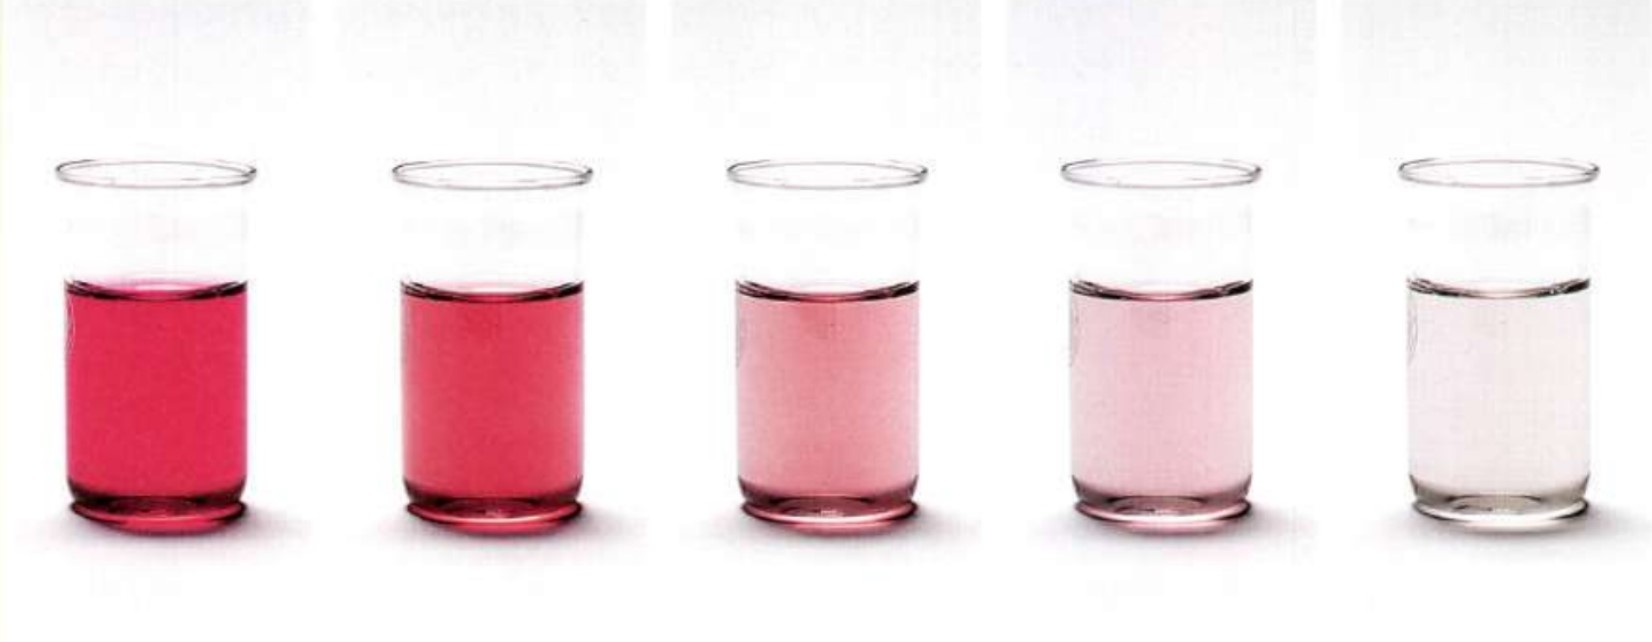
\includegraphics[width=0.65\textwidth, left]{images/figur_35_fra_basis_kemi_a.jpg}
        \caption{En opløsning af azorubin tilsættes Klorin, hvorefter opløsningens røde farve langsomt forsvinder.}
        \label{fig:billede_af_azo}
    \end{figure}
    \vspace{-2.8cm}
    $$ $$
    $$ $$
    $$ $$
    Vi starter med at undersøge, om reaktionen er af nulte orden. Måleresultaterne afbildes i et ($t$,[Azo])-diagram, se figur 36. Hvis reaktionen er af nulte orden, skal målepunkterne tilnærmelsesvis ligge langs en ret linje med negativ hældningskoefficient, jævnfør funktionsudtrykket for en nulte ordens reaktion:
    \begin{equation}
        [Azo]=-k*t+[Azo]_0 \nonumber
    \end{equation}
    Der udføres lineær regression på datasættet (t,[Azo]), og i figur 36 er den fremkomne tendenslinje indtegnet. Forskriften for tendenslinien er:
    \begin{flalign}
        \indent [Azo] = -1,22*10^{-6} \text{M/s} * \text{t} + 8,92 * 10^{-5} \text{M} && 
        r^2=0,9502 & \nonumber
    \end{flalign}
    Betragter man afbildningen, ses det, at punkterne ikke følger den lineære sammenhæng, idet målingerne ved start og slut ligger over tendenslinjen, hvorimod de midterste målinger ligger under tendenslinjen. Dette kan ikke henføres til tilfældige afvigelser. Det vurderes umiddelbart, at reaktionen \textit{ikke} er af nulte orden.
    \pagebreak
    \begin{figure}[h]
        \centering
        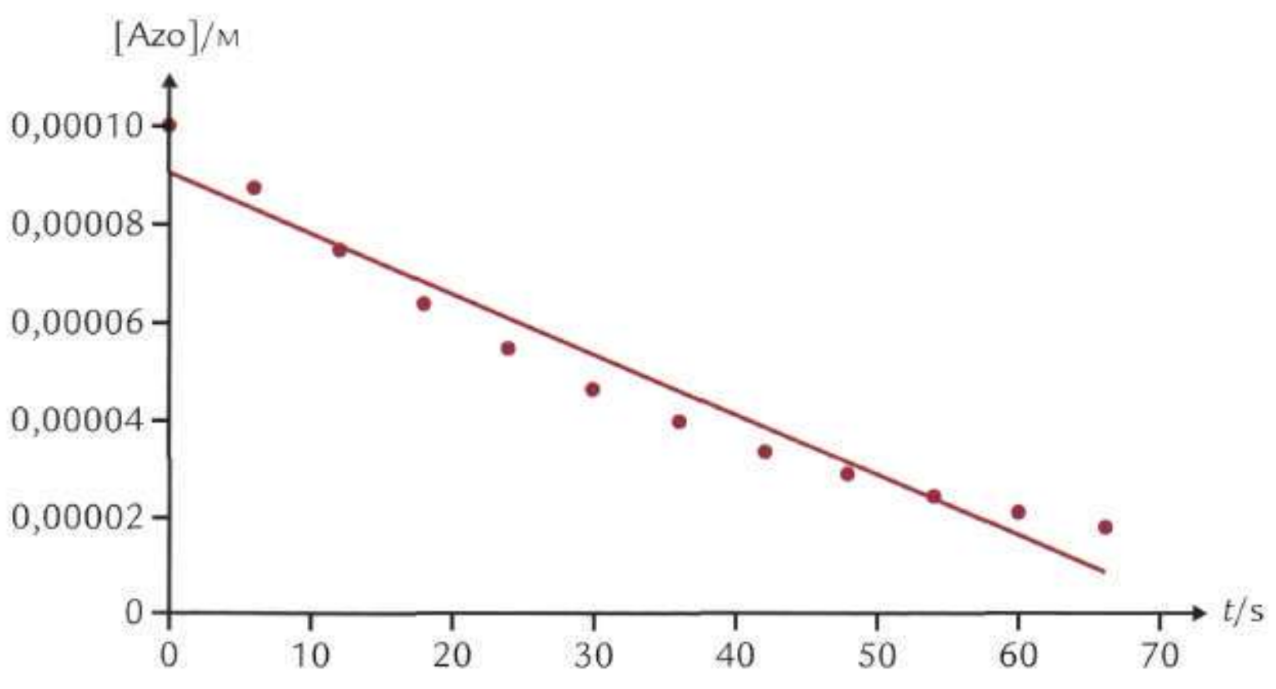
\includegraphics[width=0.7\textwidth]{images/Basiskemi_a_figur_36.png}
        \caption{Afbildning af [Azo] som funktion af tiden $t$. Der er udført lineær regression på datasættet vist i \ref{wrap-tab:Azo_table}}
        \label{fig:Azo_lineær}
    \end{figure}
    
    Vi vil nu undersøge, om reaktionen er af første orden. Der er udført eksponentiel regression på datasættet ($t$,[Azo]), jævnfør funktionsudtrykket for en første ordens reaktion:
    $$[Azo] = [Azo]_0 \, e^{-k*t}$$
    
    \begin{figure}[h]
        \centering
        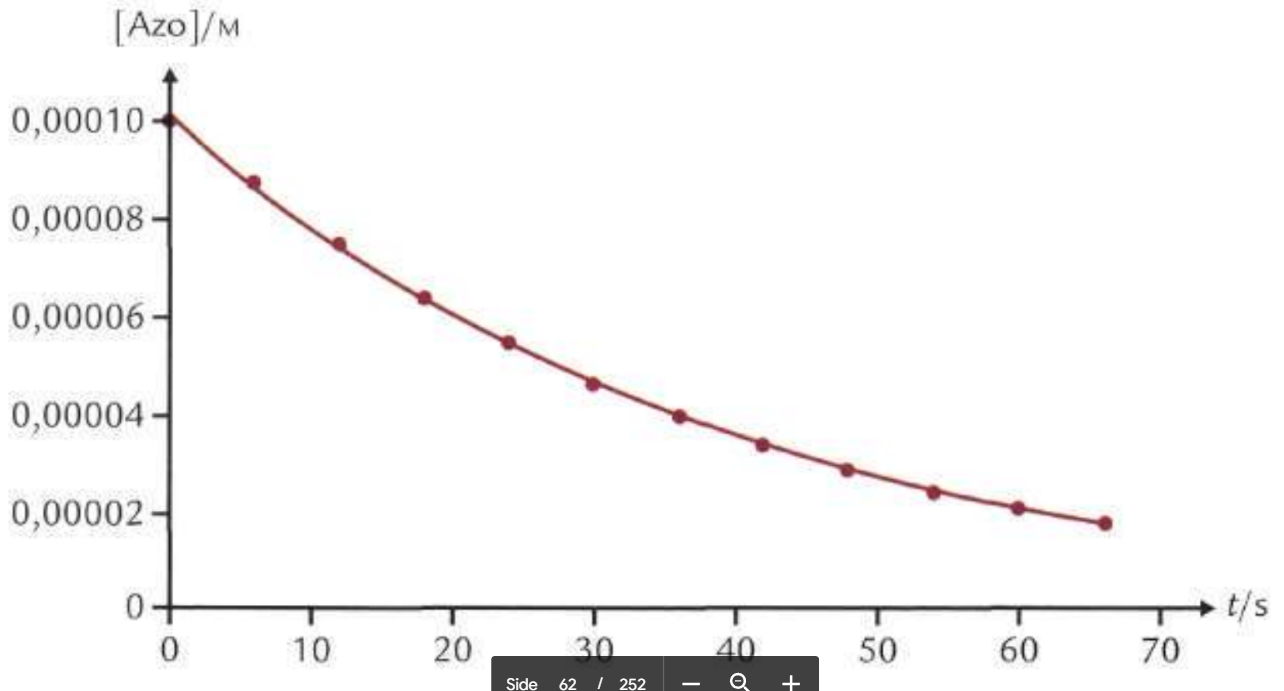
\includegraphics[width=0.7\textwidth]{images/Basiskemi_a_figur_37.png}
        \caption{Afbildning af [Azo] som funktion af tiden $t$. Det er undersøgt, om datasættet vist i \ref{wrap-tab:Azo_table} følger en eksponentiel sammenhæng.}
        \label{fig:Azo_eksponentiel}
    \end{figure}
    
    I \ref{fig:Azo_eksponentiel} er den fremkomne tendenslinje indtegnet. Forskriften for tendenslinjen er:
    \begin{flalign}
        \indent [Azo] = 1,01*10^{-4}\; \text{M} \, * e^{-0,0262 \text{s}^{-1}*\text{t}} && 
        r^2=0,9999 & \nonumber
    \end{flalign}
    Betragter man afbildningen, ses det, at punkterne næsten perfekt følger den eksponentielle sammenhæng. Der er ikke umiddelbart nogen målinger, som afviger systematisk. De små afvigelser er helt tilfældigt fordelt. Det vurderes umiddelbart, at reaktionen er af første orden. I stedet for en afbildning af ($t$,[Azo]) kan man også vælge at lave en afbildning af ($t$,ln[Azo]) og udføre lineær regression, jævnfør funktionsudtrykket:
    
    \begin{equation}
        \ln[Azo] = -k*t+\ln[Azo]_0 \nonumber
    \end{equation}
    
    \begin{figure}[h]
        \centering
        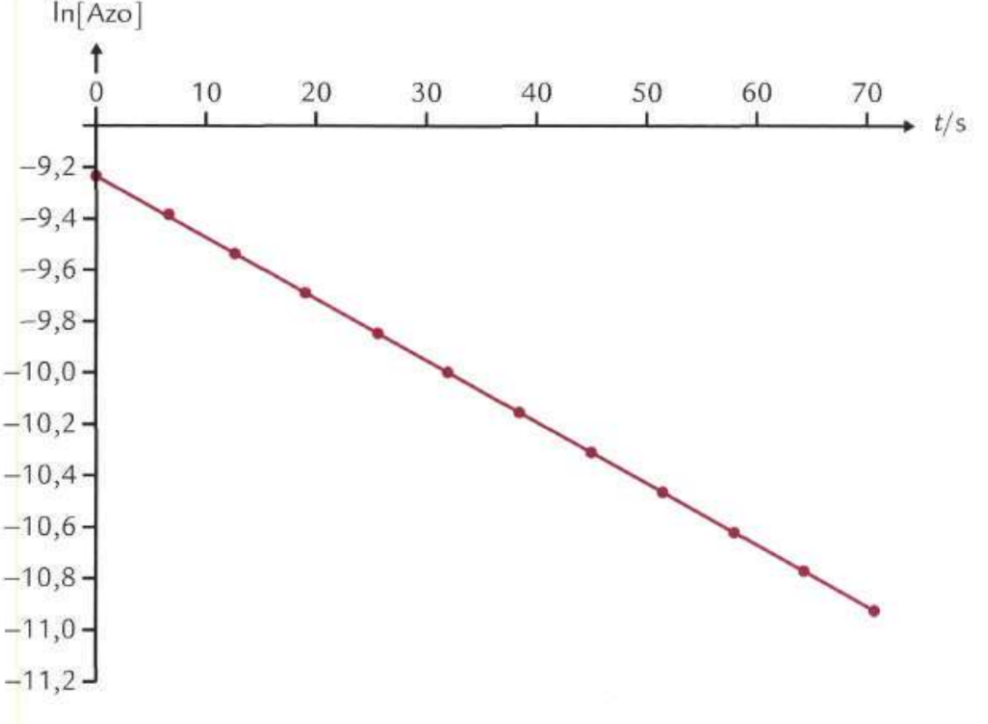
\includegraphics[width=0.55\textwidth]{images/Basiskemi_a_figur_38.png}
        \caption{Afbildning af ln[Azo] som funktion af tiden $t$. Der er udført lineær regression på datasættet}
        \label{fig:ln_Azo}
    \end{figure}
    \pagebreak
    I \ref{fig:ln_Azo} er der udført lineær regression på datasættet ($t$,ln[Azo]), og den fremkomne tendenslinje er indtegnet. Forskriften for tendenslinjen er:
    \begin{flalign}
       \indent \ln[Azo] = -0,0262\, \text{s}^{-1}*t-9,20 && 
       r^2=0,9984 & \nonumber
    \end{flalign}
    Betragter man afbildningen, ses det, at punkterne næsten perfekt følger den lineære sammenhæng. Der er ikke umiddelbart nogen målinger, som afviger systematisk. De små afvigelser er helt tilfældigt fordelt. Det vurderes naturligvis også ud fra denne type regressionsanalyse, at reaktionen er af første orden.
    For en god ordens skyld undersøger vi også, om reaktionen kunne være af anden orden. Måleresultaterne afbildes i et $(\frac{1}{[Azo]})$ diagram. Hvis reaktionen skal være af anden orden, skal målepunkterne tilnærmelsesvis ligge langs en ret linje med positiv hældningskoefficient, jævnfør funktionsudtrykket:
    
    \begin{equation}
        \indent \frac{1}{[Azo]} = k*t+\frac{1}{[Azo]_0} \nonumber
    \end{equation}
    I figur \ref{fig:reciprok_Azo} er der udført lineær regression på datasættet $(\frac{1}{[Azo]})$ og den fremkomne tendenslinje er indtegnet. Forskriften for tendenslinjen er:
    \begin{flalign}
       \indent \frac{1}{[Azo]} = 672\, \text{M}^{-1} * \text{s}^{-1}*t+4,95*10^{3}\, \text{M}^{-1} && 
       r^2=0,9481 & \nonumber
    \end{flalign}
    
    \begin{figure}[h]
        \centering
        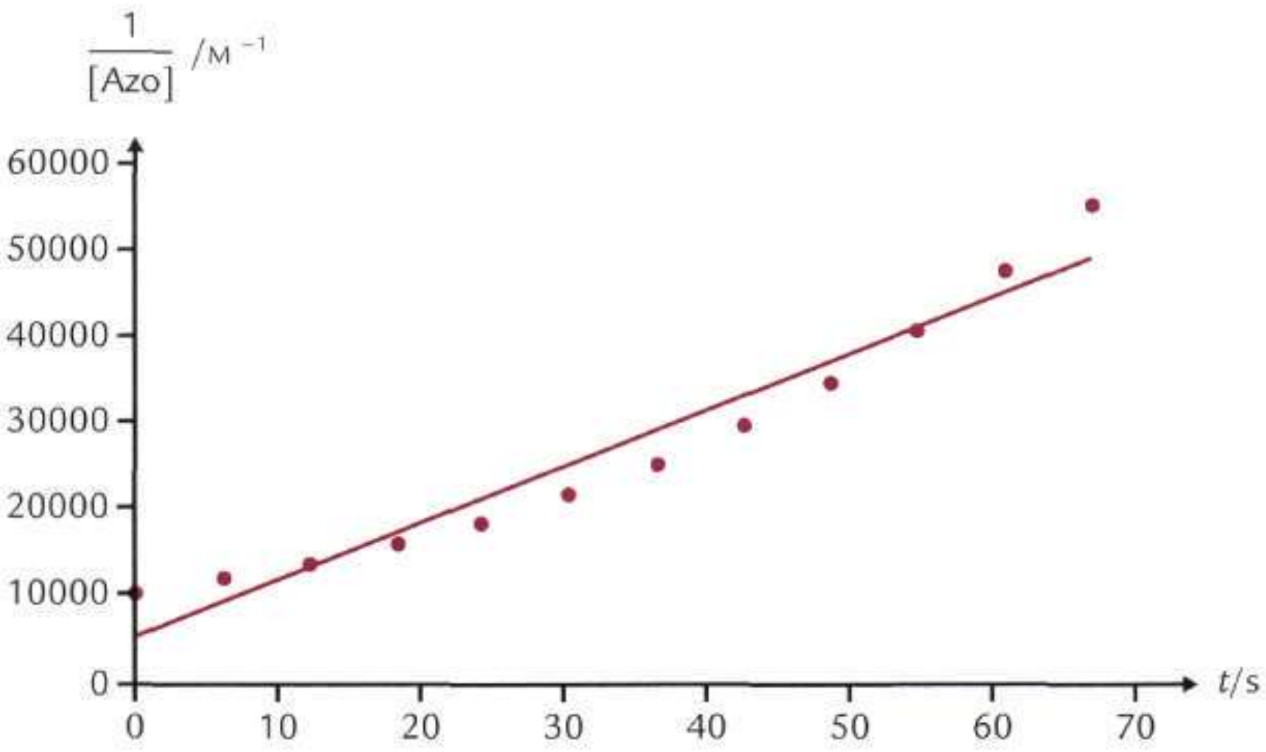
\includegraphics[width=0.55\textwidth]{images/Basiskemi_a_figur_39.png}
        \caption{Afbildning af $(\frac{1}{[Azo]})$ som funktion af tiden $t$. Der er udført lineær regression på datasættet}
        \label{fig:reciprok_Azo}
    \end{figure}
    \pagebreak
    Betragter man afbildningen, ses det, at punkterne ikke følger den lineære sammenhæng, idet målingerne ved start og slut ligger over tendenslinjen, hvorimod de midterste målinger ligger under tendenslinjen. Denne type afvigelser kan ikke henføres som tilfældige afvigelser. Det vurderes umiddelbart, at reaktionen ikke er af anden orden. Ud fra undersøgelsen kan vi konkludere, at affarvningen af azorubin i det nævnte eksperiment er en første ordens reaktion, og vi får følgende:
    
    \begin{flalign}
         [Azo] = 1,01*10^{-4} * \, \text{M} * e^{-0,0262\; \text{s}^{-1}*t} \nonumber \\ 
        \ln[Azo] = -0,0262\; \text{s}^{-1}*t*t-9,20 \nonumber
    \end{flalign}
    dvs. hastighedskonstanten for reaktionen er $k = 0,0262 \text{s}^{-1}$ Hastighedsudtrykket for affarvningen af azorubin kan nu opskrives:
    \begin{flalign}
        v = -0,0262\; \text{s}^{-1}*[Azo] \nonumber
    \end{flalign}
    Andre faktorer kan have indflydelse på hastighedsudtrykket, fx surhedsgrad, stofmængdekoncentrationen af hypochlorit i den anvendte Klorin og temperaturen. Det vil kræve yderligere undersøgelser at klarlægge disse faktorers betydning.\\\\
    

    
\newpage
\twocolumn
\chapter{Spektroskopi}
\section{Formler}

\begin{table}[]
    \begin{tabular}{ l l l}
    \multicolumn{3}{l}{\textbf{Spektroskopi}} \\
        \hline  
        $A$ & absorbans & $(\text{ingen})$ \\
        $\varepsilon_\lambda$ & absorptionskoefficient & \\
        $ $ & (ekstinktionkoeffcient) & $(\text{M}\inv * \text{cm}\inv$ \\ 
        $ $ & $ $ & = $\text{L}/(\text{mol}*\text{cm}))$ \\
        $l$ & lysvej (kuvettebredde) & $(\text{cm})$ \\
        $E$ & energi & $(\text{J})$ \\
        $f$ & frekvensen & $(\text{Hz}=\text{s}\inv)$ \\
        $c$ & lysets fart & $(\text{m}/\text{s})$ \\
        $\lambda$ & bølgelængde & $(\text{m})$ \\
        $\tau$ & transmittans & $(\text{ingen, \%})$ \\
        $\lambda ^{-1}$ & bølgetal & $(\text{cm}\inv)$ \\
        $\delta$ & kemisk skift & $(\text{ingen, ppm})$ \\
        $J$ & koblingskonstant & $(\text{Hz})$ \\
    \end{tabular}
    \caption{Symboler og deres enheder}
    \label{tab:spektroskopi_table}
\end{table}

\begin{flalign}
    A = \varepsilon_\lambda * [A] * l &&
\end{flalign}
Lambert-Beers lov. Når lys sendes gennem en opløsning af et stof $A$, er absorbansen lig med produktet af den molare absorptionskoefficient (ekstinktionskoefficient), stoffets aktuelle koncentration og lysets vejlængde (kuvettebredden) gennem stoffet.

\begin{flalign}
    E_{foton} = h * f &&
\end{flalign}
En fotons energi er lig med produktet af Planck-konstanten og lysets frekvens

\begin{flalign}
    E_{foton} = E_{høj} - E_{lav} &&
\end{flalign}
Den foton, der udsende ved en overgang fra en stationær tilstand med energien $E_{høj}$ til en overgang med energien $E_{lav}$ er lig med forskellen i energi mellem de to tilstande. 

\begin{flalign}
    c = \frac{\lambda}{f} &&
\end{flalign}
Lysets udbredelsesfart er lig med produktet af lysets bølgelængde og lysets frekvens.

\begin{flalign}
    \tau = \frac{I}{I_0}&&
\end{flalign}
Transmittansen er lig med forholdet mellem intensiteten af strålingen efter absorption divideret med intensiteten af strålingen før absorption

\begin{flalign}
    \delta = \frac{f_{resonans} - f_{TMS}}{f_{TMS}} &&
\end{flalign}
Det kemiske skift for en resonanslinje er lig med den relative forskydning af linjens resonansfrekvensen i forhold til resonansfrekvensen for tetramethylsilan, TMS. 

\begin{flalign}
    J_{ax} = f_{NMR} * \Delta \delta &&
\end{flalign}
Koblingskonstanten er lig med produktet af NMR-spektrometerets frekvens og forskellen i kemisk skift. 

\begin{flalign}
    DBE = \frac{(2c+2)-(h-n)}{2} &&
\end{flalign}
Antallet af dobbeltbindingsækvivalenter i et organisk molekyler kan beregnes ud fra den viste formel, $c$ er antallet af carbonatomer, $h$ antallet af hydrogenatomer og $n$ er antallet af nitrogenatomer. 
\newpage
\onecolumn


\chemfig{H-C(-[2]H)(-[6]H)-C(-[0]H)(-[2]H)-[6]H}



\newpage

\quickwordcount{main}
\quickcharcount{main}

There are \thechar characters and approximately \theword spaces.
That makes approximately \the\numexpr\theword+\thechar\relax\ characters total.

\end{document}